\chapter{Dynamic plant--soil microbe interactions: the neglected effect of soil conditioning time}
%\chaptermark{Positive frequency-dependence}
%\renewcommand{\sectionmark}[1]{}
\fancyhead[LE, RO]{\thepage}
\fancyhead[RE]{CHAPTER 6}
\fancyhead[LO]{TEMPORAL PLANT--SOIL FEEDBACK}
\fancyfoot{}
\renewcommand{\headrulewidth}{0pt}
\setlength{\parindent}{1cm}



\begin{comment}
\documentclass[hidelinks,letterpaper, 11pt]{article}
\usepackage{graphicx, bm, booktabs, lineno, array}
\usepackage[fleqn]{amsmath}
\usepackage{nicefrac}
\usepackage[compress,comma]{natbib}
\usepackage[right=1in, left=1in, top=1in, bottom=1in]{geometry}
\usepackage[parfill]{parskip}
\usepackage[usenames,dvipsnames]{color}
\usepackage[font=large,labelfont=bf,margin=1cm, labelsep = none]{caption} % caption formatting
\usepackage{setspace}
\usepackage{gensymb}
\usepackage{color}
\usepackage{sidecap}
%\usepackage{floatrow}
\usepackage{etoolbox}
\usepackage{tcolorbox}
\usepackage{newpxtext,newpxmath}
\tcbuselibrary{breakable}
%\usepackage{indentfirst}
\newbool{MyRefNumbers}
\usepackage{authblk}
\usepackage{hyperref}
\usepackage{mathpazo}
\usepackage[color=cyan, textsize=tiny]{todonotes}
\usepackage[font={normalsize}]{caption}
\usepackage{adjustbox}
\usepackage{array}
\usepackage{booktabs}
\usepackage{multirow}
\usepackage{tabularx}
% \usepackage{titling}

\setlength{\mathindent}{0pt}
\setlength{\parindent}{1cm}
% \makeatletter
% \makeatother
\pdfminorversion=3

% For table
\newenvironment{myindentpar}[1]%
{\begin{list}{}%
		{\setlength{\leftmargin}{#1}}%
		\item[]%
	}
	{\end{list}}
\newcommand*\samethanks[1][\value{footnote}]{\footnotemark[#1]}
\newcommand\blfootnote[1]{%
	\begingroup
	\renewcommand\thefootnote{}\footnote{#1}%
	\addtocounter{footnote}{-1}%
	\endgroup
}
\newcommand{\plus}{\raisebox{.4\height}{\scalebox{.6}{+}}}
\newcommand{\minus}{\raisebox{.4\height}{\scalebox{.8}{-}}}
% Command to recount supplement
\newcommand{\beginsupplement}{%
	\setcounter{table}{0}
	\renewcommand{\thetable}{S\arabic{table}}%
	\setcounter{figure}{0}
	\renewcommand{\thefigure}{S\arabic{figure}}%
}
% Command to center oversized images in floats
\newcommand{\centerfloat}{%
	\parindent \z@
	\leftskip \z@ \@plus 1fil \@minus \textwidth
	\rightskip\leftskip
	\parfillskip \z@skip}
\renewcommand\Affilfont{\fontsize{12}{12}\selectfont}
\newcommand{\ignore}[2]{\hspace{0in}#2}
\end{comment}



\begin{comment}
\begin{document}

\doublespacing
\title{Dynamic plant--soil microbe interactions: \\ the neglected effect of soil conditioning time}
\author[1, $\dagger$]{Po-Ju Ke}
\author[2]{Peter C. Zee}
\author[1, $\dagger$]{Tadashi Fukami}
\affil[1]{Department of Biology, Stanford University, Stanford, California, 94305, USA}
\affil[2]{Department of Biology, University of Mississippi, University, Mississippi, 38677, USA}
\date{\today}
\maketitle
\blfootnote{$\dagger$ Correspondence author: Department of Biology, Stanford University, Stanford, California 94305-5020, USA. Phone: +1 650-721-1711. Fax: +1 650-723-6132. Email: pojuke@stanford.edu, fukamit@stanford.edu}
	
\onehalfspacing
\noindent \textbf{Running title:} Temporal development of plant--soil feedback\\
\noindent \textbf{Keywords:} aerial photos, chronosequence, microbial community, plant--soil feedback, sand dunes, space-for-time substitution\\
\noindent \textbf{Type of article:} Letter\\
	
\begin{myindentpar}{1cm}
	\textbf{Words in Abstract:} 150\\
	\textbf{Words in main text:} $\sim$ 4000\\
	\textbf{Number of references:} 63\\
	\textbf{Number of figures:} 5\\
\end{myindentpar}
	
\noindent \textbf{Authorship statement:} PJK and TF conceived the study; PJK conducted the study and analyzed the data; PJK and PCZ developed the model and performed the simulation; PJK wrote the first draft of the manuscript with substantial contribution from all authors.\\
	
\noindent \textbf{Data accessibility statement:} Should the manuscript be accepted, all data and computer scripts supporting the results will be archived in a public Github repository, with the DOI included at the end of the article.\\

\linenumbers
\doublespacing
\end{comment}



\section{Abstract}
Plant--soil feedbacks (PSF), the reciprocal interactions between plants and soil microbes, shape the structure of plant communities, but how the length of soil conditioning affects PSF strength is rarely studied. 
Using a chronosequence reconstructed from aerial photos, we characterized the soil microbial communities associated with four perennial dune plants and their turnover as plants aged. 
We also quantified PSF strength in a greenhouse experiment that preserved age-specific soil properties.
For all plants, we found that their microbial communities changed with increasing conditioning time.
The greenhouse experiment showed that these compositional turnovers caused PSF strength to change in ways that depended on the specific plant--soil combination. 
With an individual-based simulation model, we further found that the temporal development patterns of PSF affected the rate of plant community convergence. 
Taken together, we suggest that future studies should consider the temporal development pattern of PSF to understand its effects on plant community assembly.
\medskip


\noindent \textbf{Keywords:} aerial photos, chronosequence, microbial community, plant--soil feedback, sand dunes, space-for-time substitution



\section{Introduction}
%Plant-soil interactions are important and assumed to be constant
It is widely recognized that interactions between plants and soil microbes, known as plant--soil feedbacks (PSF), can affect the structure of plant communities \citep{Bever2010, vanderPutten2013, KeMiki2015}. 
Plants cause changes in the composition of the soil microbial community, which then feeds back to affect the growth of neighboring plants \citep{Bever1997, Bever2003}. As plant species vary in their response to soil microbes, PSF can modify differences in plant performance and alter plant community composition \citep{Klironomos2002, Mangan2010, Eppinga2018}.
The strengths of these feedbacks are commonly assumed to be constant through time \citep{Kardol2013}. Under this assumption, most empirical studies quantify feedback strengths via short-term greenhouse experiments that are terminated at the same time for all species \citep{KulmatiskiKardol2008, Kardol2013}. The estimated feedback strengths are then incorporated into theoretical models as time-independent parameters (e.g., \citealp{Fukami2013, Bauer2015, Teste2017}). 
\par


%The importance of a dynamic PSF viewpoint
Recent studies have started to recognize that PSF strength can vary across plant life stages due to ontogenetic changes in plant's responses to soil microbes \citep{Hawkes2012, Dudenhoffer2017, Bezemer2018}. 
Temporal development of PSFs can also be driven by changes in microbial community composition with plant age (i.e., the duration of soil conditioning), which proceeds at different rates depending on host plant identity \citep{Knelman2012}. 
Explicit consideration of the effects of soil conditioning length, however, is lacking in the current PSF literature probably owing to two logistical challenges. First, preparing soils with different conditioning lengths is often not feasible in the greenhouse \citep{Kardol2013, Kulmatiski2018}, and second, the length of soil conditioning in the field can only be quantified with coarse resolution due to uncertainty about the ages of individual plants (e.g., \citealp{Speek2015, Day2015}).
\par


%Aim of paper
In this paper, we study how PSF strengths vary with the length of soil conditioning and how the temporal patterns differ among plant species. 
To this end, we used high-resolution aerial photos of the coastal dune vegetation at Bodega Bay in California, which were taken annually from 1992 to 2016. This unique resource allowed us to estimate the age of individual plants and use it as a proxy for soil conditioning length. 
By sampling soils from individual plants of different ages, we applied a chronosequence approach to examine how soil microbial communities vary across plant species and conditioning time. We then designed a greenhouse experiment that preserved plant age-specific microbial communities to study how changes in their composition affected species' PSF strength.
This combination of approaches allowed us to overcome the logical challenges outlined above and study the link between plant age, soil microbial composition, and feedback strength. 
Finally, we used a general individual-based simulation model to explore how the temporal pattern of PSF may affect plant community assembly and their transient dynamics.
\par



\section{Methods}
\subsection*{Study system}
%Basic information and natural history of Bodega bay 
We conducted our study at the coastal foredunes of Bodega Bay, California, USA (38$^{\circ}$19$^\prime$ N, 123$^{\circ}$3$^\prime$ W), located within UC Davis Bodega Marine Reserve and Sonoma Coast State Beaches. This region experiences a Mediterranean-type climate, with an average annual temperature of 15.8$^{\circ}$C and annual precipitation of 760 mm, mostly occurring between October to April \citep{Barbour1973, Conser2009}. The soils in our 400 $\times$ 500 m study area are predominantly sand, with a negligible amount of silt and clay \citep{Kleinhesselink2014}. 
We focused on the four dominant species of the foredune plant community, including the introduced grass \textit{Ammophila arenaria} (Poaceae), the introduced succulent dwarf-shrub \textit{Carpobrotus edulis} (Aizoaceae), and the native shrubs \textit{Baccharis pilularis} (Asteraceae) and \textit{Lupinus arboreus} (Fabaceae). 
\par



\subsection*{Soil sampling}
%Plant individual selection
We used a series of aerial photos that were taken annually by Delta Geomatics Corporation, and curated by the Bodega Marine Reserve, from 1992 to 2016 \citep{Danin1998}. Since the foredune vegetation has little vertical structure, we were able to identify plant individuals to the species level and estimate their age (i.e., identify the first year the individual appeared in the photos) by comparing photos across multiple years. Age estimates were used as proxies for soil conditioning length as the foredune undergoes primary succession starting from unconditioned bare sand. 
For each of the four dominant species, we selected 30 individuals of different ages along the chronosequence. All individuals were selected to sample evenly along the plant's age span provided by the aerial photos, which ranged between 1 to 11 years for \textit{L. arboreus} and between 2 to 25 years for the other three species.
No spatial autocorrelation was evident for the age of selected individuals (Moran's I, $P = 0.24$; Mantel test, $P = 0.39$). 
See Fig.~\ref{fig:map} for a representative aerial photo, the spatial distribution of selected individuals, and representative examples of different age classes for each species.
\par


%Soil sampling for microbial community patterns
To study how soil microbial communities varied with plant age, in July 2016 we collected three soil samples beneath each plant individual (i.e., at azimuth angles 0$^{\circ}$, 120$^{\circ}$, and 240$^{\circ}$) in separate sterile 50 mL Falcon tubes. 
An additional 3 and 13 individuals of \textit{C. edulis} and \textit{L. arboreus}, respectively, were sampled for this microbial community survey. We also collected soil samples from three randomly selected juveniles (i.e., one sample per juvenile, which are individuals that germinated within one year and were too small to be visible on the aerial photos from the previous year) for three of the four species (i.e., all but \textit{A. arenaria}). Finally, a total of 13 soil samples from randomly selected bare sand areas (i.e., no vegetation in an approximately 3 m radius throughout the entire length of time of the aerial photos) were collected across our field site (Fig.~\ref{fig:map}). 
All soil samples were stored at 4$^{\circ}$C before being processed in the lab. Within one week after collection, soil samples were processed by passing through a sterile 2 mm mesh sieve and homogenized thoroughly in separate sterile plastic bags.
The fungal and bacterial communities of the resulting 430 soil samples (i.e., 136 individuals $\times$ 3 samples + 3 species $\times$ 3 juveniles + 13 bare sand samples) were characterize with next-generation sequencing (see section `\textit{DNA sequencing of fungal and bacterial communities}').
\par



\subsection*{DNA sequencing of fungal and bacterial communities}
%Brief overview of NGS flow
For each processed soil sample collected in July 2016, we extracted microbial DNA from 0.25 g of subsampled soil with the PowerSoil DNA Isolation Kit. We then PCR-amplified the bacterial 16S ribosomal DNA region and the fungal internal transcribed spacer 1 region (ITS1) with specific primer pairs \citep{Caporaso2012, Toju2012, Lundberg2013, Hamady2008}. Amplicon libraries were then normalized, pooled, sequenced by the Illumina MiSeq sequencer, and processed through a bioinformatic pipeline \citep{Wang2007, Edgar2011, McMurdie2013, Tanabe2013, Zhang2014, Deshpande2016, Rognes2016, Davis2018} to obtain a rarefied sample $\times$ operational taxonomic units (OTUs) matrix. See Appendix E.1 for detailed description.
\par



\subsection*{Greenhouse experiment}
To examine changes in the effects of soil microbial communities on plant performance in a greenhouse experiment, we revisited the same plant individuals in July 2017. 
For all four species, we collected 300 mL of soil from each individual within a random subset of previously sampled individuals ($N = 27$). Soils were collected, and pooled together, from three positions adjacent to the original sampling position in 2016 (100 mL from each position using a sterile soil core sampler). We also collected the same amount of soil from three new randomly selected juveniles for all four species. 
Soils collected from all 120 individuals (i.e., 4 species $\times$ 27 individuals + 4 species $\times$ 3 juveniles) were processed with the same method as above and stored at 4$^{\circ}$C before the greenhouse experiment.
\par


%Soil preparation for the greenhouse experiment
Our greenhouse experiment used soil samples collected in July 2017 and was performed in two separate rounds, which started in late August and September 2017, respectively.
Soils collected from different plant individuals were kept separated throughout the experiment so that each soil maintained its age-specific properties \citep{Rinella2018}.
The range and variance of plant individual age were kept similar among the two experiment rounds (i.e., by sorting individuals based on their age and assigning every other individual along the age axis to different experiment round). 
Half of the soil volume collected from each individual was autoclaved to create a sterile treatment, allowing us to isolate the effects of soil microbial communities. 
Soils collected from 9 individuals were discarded due to handling mistakes (i.e., 6 and 3 individuals for the first and second round, respectively), resulting in a total of 222 unique soil environments that differed in their host plant species, individual age, and sterilization treatment (i.e., 111 individuals $\times$ 2 sterilization treatments).
\par


%Seedling transplant for the greenhouse experiment
Seeds of the four species were surface-sterilized and allowed to germinate on autoclaved sand under controlled condition (see Appendix E.1). After two weeks, we transplanted the seedlings individually into 107 mL ``cone-tainer'' pots (i.e., one seedling per pot) filled with 80 mL of sterilized sand and added 20 mL of either live or sterile soil inoculum to the top. 
Our experiment examined the full combination of transplanting each of the four species into all 222 soil environments. However, \textit{B. pilularis} was omitted during the second round due to low germination rate, resulting in a total of 774 pots (i.e., 432 in the first round (54 individuals $\times$ 2 sterilization treatments $\times$ 4 species) and 342 in the second round (57 individuals $\times$ 2 sterilization treatments $\times$ 3 species); see Appendix E.1 for detail).
Seedlings grew in the greenhouse for 12 weeks, after which we harvested and oven-dried all plant tissues from each pot at 70$^{\circ}$C for 96 h. The resulting total dry biomass was weighed to quantify the effects of soil microbes on plant performance.
\par



\subsection*{Data analysis}
%Distance-based community level analysis for microbial communities
We analyzed the fungal and bacterial communities separately. To better match our microbial community data from soil samples to the soils used in our greenhouse experiment, we summed the OTU reads of the three samples that belonged to the same plant individual. As a result, the following statistical analyses were performed by viewing plant individuals as the unit of replication. 
To examine how alpha diversity of the microbial community varied with plant age, we fitted linear, quadratic, and Monod functions (with R package nlme) to model ln(observed OTU richness) as a function of plant age. Models were fitted for each plant species separately, and the best model was selected based on their AICc values.
To visualize compositional differences among microbial communities, we used non-metric multidimensional scaling (NMDS) to ordinate microbial communities based on Bray-Curtis dissimilarity matrices (with R packages vegan and phyloseq). Effects of soil host species identity and plant age on microbial community composition were tested with permutational multivariate analysis of variance (PERMANOVA with 999 permutations, \citealp{Anderson2011}). 
To identify the microbial taxonomic groups that drove the observed community pattern, we aggregated the microbial communities to the family level and modeled the abundance of each family as a function of plant age using the R package HMSC (\citealp{Ovaskainen2017}, see Appendix E.1 for detail). 
Note that all statistics with plant age as a predictor were performed for each plant species separately. This is because species vary in their longevity and thus the same age does not necessarily represent the same life stage for different species.
\par


%Defining our PSF index
In our greenhouse experiment, seedlings of the same plant species were paired based on the plant individual where field soils were collected, with one seedling inoculated with live soil and the other with sterile soil from the same plant individual. As soils from different individuals were not mixed \citep{Rinella2018}, we were able to quantify the effects that the soil microbial community from a $k$-year-old individual of species $j$ (denoted as the $j^{k}$ individual) had on species $i$ as:

\begin{equation}
\sigma_{i, \,j^{k}} = \textup{log}_{10}(\frac{B_{i, \,j^{k}, \,live}}{B_{i, \,j^{k}, \,sterile}}), \nonumber
\end{equation}

\noindent where $B_{i, \,j^{k}, \,live}$ and $B_{i, \,j^{k}, \,sterile}$ represent seedling biomass of species $i$ when grown in soils inoculated with either live or sterile soil from the $k$-year-old individual of species $j$, respectively. Since the inocula used in the two biomass measurements were collected from the same plant individual in the field, the resulting metric is an ``age-specific microbial effect'' associated with the $j^{k}$ individual. A positive (or negative) value means that the soil microbial community associated with the $j^{k}$ individual had a net beneficial (or detrimental) effect on the seedling of species $i$. For this paired calculation, data for 20 live--sterile soil pairs were discarded due to seedling death or handling mistakes. 
\par


%Statistical tests with the PSF index  -- static perspective
We used two approaches to analyze the age-specific microbial effects. First, we took the time-averaged value of $\sigma_{i, \,j^{k}}$ for each plant $\times$ soil host species combination (i.e., ignored the age information by taking the temporal mean), which is the common approach used in studies when the information of soil conditioning length is not available. 
For each of the four plant species, the effects of soil host species on the time-averaged microbial effect were tested by fitting generalized linear mixed models (GLMM, with normal distribution of errors using R package lme4). We included the identity of soil host species as a fixed effect and greenhouse round, when present, as a random effect. Post-hoc group comparisons with Holm--Bonferroni adjusted probabilities were performed (with R package multcomp).
For each of the 16 plant $\times$ soil host species combinations, an additional \textit{t}-test was used to test if the time-averaged microbial effect was significantly different from zero.
\par
 
 
%Statistical tests with the PSF index  -- dynamics perspective
The second approach took advantage of the age information provided by the aerial photos. Specifically, we visualized the age-specific microbial effects on the temporal axis (i.e., soil conditioning length) and quantified the temporal development pattern for each of the 16 plant $\times$ soil host species combinations.
We applied a two-step process to test if the strength of microbial effects varied with increasing conditioning time. First, we fitted separate GLMMs with plant age as a fixed effect and greenhouse round as a random effect for each of the 16 plant $\times$ soil host species combinations. For this step, we fitted both linear and quadratic functional forms and selected the best model based on their AICc values. 
Second, for temporal patterns that were not statistically significant, we fitted a Monod function to assess how fast the microbial effects would build up. If both steps of the fitting procedure resulted in a poor model fit (i.e., age had no significant effects, and the nonlinear Monod fitting procedure failed to converge), we concluded that the length of soil conditioning had little influence on the microbial effect for this plant $\times$ soil host species combination. All analyses and simulations were performed in \textit{R} version 3.3.1 \citep{R}. 
\par



\subsection*{Simulation model}
To further study how the temporal development of PSF affects plant community assembly, we constructed a general individual-based model following \citet{FukamiNakajima2011} (see also \citealp{Fukami2013, ZeeFukami2015, Fukami2017}). 
% We constructed a general individual-based model following \citet{FukamiNakajima2011} (see also \citealp{Fukami2013, ZeeFukami2015, Fukami2017}). 
Our simulation exercise focuses on both transient and steady states of plant community assembly and explores the potential consequences of different temporal development patterns of PSF.
The model consists of species pools containing 50 species (each with a different trait value) and patches consisting of 1024 local sites (each with a different habitat conditions). We simulated the processes of immigration, reproduction, arrival, competition for establishment, and death of plant individuals. 
Competition for establishment at empty sites is determined not only by the match between species' trait values and local habitat conditions (i.e., environmental filtering) but also by the soil microbial legacy effects (i.e., PSF) created by the previously established plant species. 
Based on empirical evidence, we allowed the microbial legacy effects to be either positive or negative (i.e., complex feedback regime, \textit{sensu} \citealp{Fukami2013}).
The key distinction between our model and previous studies is that microbial legacy effects in our model are age-dependent, i.e., the strength depends on the age of death of the previous established individual. See Appendix E.1 for full details of the simulation model.
\par


For our simulation, we generated 10 patches for the regional species pool to colonize independently and one set of baseline microbial legacy effects, which represent the microbial effects created by the previous individual if it died a year immediately after colonization.
The microbial effects experienced by a new arriving species depends on the previous individual's age of death and the temporal development pattern of microbial effects.
Here, we considered four scenarios: (1) `constant', where microbial effects remain unchanged despite individuals becoming older; (2) `magnifying', where both positive and negative microbial effects intensify in strength as individuals become older (i.e., the longer the previous individual lived before it died, the stronger its impact on the new individual); (3) `decaying', where both positive and negative microbial effects attenuate in strength as individuals become older; and (4) `bidirectionally varying', where both intensifying and attenuating are possible. 
For each scenario, we simulated 20 replicated runs of community assembly, where 20 independently created sets of species pool (each with 50 species) were allowed to colonize the same set of 10 patches, using the same set of baseline microbial effects. 
We quantified the beta diversity among the 10 patches for each replicated run, which is measured as the gamma diversity divided by the mean alpha diversity, and compared the temporal patterns of beta diversity among different scenarios.
\par



\begin{comment}
% PBA-1: This comes out of the blue a little. Needs better motivation. (DONE: changed the motivation sentence)
% PBA-2: I was also left wondering why you don't seem to use your field data to inform this model, shouldn't the temporal patterns of PSF development match your field results? (CANNOT DO) 
% PBA-3: And why is community convergence the key response? Rather than something like richness or abundance distribution? (CONE: it's actually the only meaningful comparison in this model, downplayed it term) 
% EGM-1: Why didn’t you simply parameterize the model using the empirical PSF measurements for your 4 species, and simulate the dynamics through time? Some justification of this approach is needed. (CANNOT DO)
% EGM-2: Again, justify this decision because it seems very arbitrary. Why not use all 50 species in the community assembly simulation, for example? (CAN DO: clarify this specific question about the generation of replicated species pool)
\end{comment}


% We simulated 20 replicated runs of community assembly, where 20 independently created sets of species pool (each with 50 species) were allowed to colonize the same set of 10 patches, using the same set of microbial legacy effects. Following our empirical results, we allowed the microbial legacy effects to be either positive or negative (i.e., complex feedback regime, \textit{sensu} \citealp{Fukami2013}). For all microbial effects created by the previously established individual, four temporal development scenarios were considered: (1) `constant', where microbial effects remain unchanged despite individuals becoming older; (2) `magnifying', where both positive and negative microbial effects intensify in strength as individuals become older (i.e., the longer the previous individual lived before it died, the stronger its impact on the new individual); (3) `decaying', where both positive and negative microbial effects attenuate in strength as individuals become older; and (4) `bidirectionally varying', where both intensifying and attenuating are possible. For each scenario, we quantified the beta diversity among the 10 patches for replicated run, which is measured as the gamma diversity divided by the mean alpha diversity, and compared the temporal patterns of beta diversity (i.e., detecting community convergence or divergence) among different scenarios.



\section{Results}
\subsection*{Temporal patterns of microbial communities}
Fungal community composition differed among plant species (Fig.~\ref{fig:BothComposition}a, PERMANOVA, $R^{2}=0.148$, $P<0.001$). Within each plant species, fungal composition varied with plant age (Fig.~\ref{fig:FunComposition}, age effect for \textit{A. arenaria}: $R^{2}=0.096$; \textit{B. pilularis}: $R^{2}=0.083$; \textit{C. edulis}: $R^{2}=0.100$; \textit{L. arboreus}: $R^{2}=0.077$; all $P<0.001$) and became progressively different from bare sand communities with increasing conditioning time (fungal richness ceased to increase further after a few years following plant colonization, Fig.~\ref{fig:FunRichness}).
Similar results were observed for bacterial communities (Figs.~\ref{fig:BothComposition}b, \ref{fig:BacRichness}, and \ref{fig:BacComposition}, species effect: $R^{2}=0.126$; age effect for \textit{A. arenaria}: $R^{2}=0.115$; \textit{B. pilularis}: $R^{2}=0.112$; \textit{C. edulis}: $R^{2}=0.120$; \textit{L. arboreus}: $R^{2}=0.116$; all $P<0.001$). 
Fungal and bacterial families responded differently to increasing plant age, and the temporal changes of a family depended on the identity of the plant species (Figs.~\ref{fig:FunHMSC} and \ref{fig:BacHMSC}). 
\par



\subsection*{Temporal patterns of soil microbial effects on plant performance}
%Time-averaged PSF index -- static perspective
By quantifying the time-averaged microbial effects that each plant species experienced when grown in soils conditioned by different soil host species, we found that the effects of soil microbes were largely determined by the seedling's species identity.
In particular, the microbial effects was positive for \textit{L. arboreus} but negative for the other three species (Fig.~\ref{fig:PSFBar}). 
Most microbial effects were significantly different from zero ($P<0.05$; expect for \textit{B. pilularis} when grown in soils from \textit{A. arenaria} and \textit{L. arboreus} individuals; Fig.~\ref{fig:PSFBar}b), but the identity of the soil host species had little effect on the microbial effects that plants experienced (soil host species effect for \textit{A. arenaria}: $F_{3, 103.05}=0.39$, $P=0.76$; \textit{B. pilularis}: $F_{3, 45}=0.27$, $P=0.27$; \textit{C. edulis}: $F_{3, 97.18}=2.07$, $P=0.11$; Fig.~\ref{fig:PSFBar}a--c). The only exception was \textit{L. arboreus}, which grew best in soils from \textit{C. edulis} individuals and worst in soils from \textit{A. arenaria} individuals (soil host species effect: $F_{3, 103.07}=3.55$, $P=0.02$; Fig.~\ref{fig:PSFBar}d).
\par


%Temporal development of PSF index -- dynamic perspective
Despite little effect of the soil host species identity on the time-averaged microbial effects, the temporal development pattern of the microbial effects depended on the plant $\times$ soil host species combination (Fig.~\ref{fig:PSFTemporal}). 
For example, \textit{A. arenaria} and \textit{C. edulis} experienced stronger negative microbial effects when grown in conspecific soils with a longer conditioning history (Fig.~\ref{fig:PSFTemporal}a and k). However, temporal patterns were different when these two introduced species grown in heterospecific soils conditioned by each other: the negative microbial effects that \textit{A. arenaria} imposed on \textit{C. edulis} intensified through time (Fig.~\ref{fig:PSFTemporal}i), whereas no significant temporal pattern was detected for the opposite pair (Fig.~\ref{fig:PSFTemporal}c).
The positive microbial effects that \textit{L. arboreus} experienced were instantaneous (Fig.~\ref{fig:PSFTemporal}m--o), and the microbial effects that \textit{L. arboreus} imposed on conspecies and \textit{C. edulis} did not show statistically significant temporal patterns (Fig.~\ref{fig:PSFTemporal}l and p).
\par



\subsection*{Effects of temporally varying soil microbial effects on plant community assembly}
%Simulation results
Simulation results showed that plant communities converged in all scenarios, i.e., beta diversity declined through time, as communities became dominated by a subset of species. Despite eventually reaching similar beta diversity value, simulations ran under different temporal development scenarios converged with different rates (Fig.~\ref{fig:SimulationComplexPSF}a). Similar to a previous study \citep{Fukami2013}, beta diversity declined most rapidly when plants did not create microbial legacies (Fig.~\ref{fig:SimulationComplexPSF}b; light gray line in Fig.~\ref{fig:SimulationComplexPSF}a), but was maintained at high levels and declined at slower rates if plants created microbial legacies that maintained a constant strength as individuals became older (Fig.~\ref{fig:SimulationComplexPSF}c; black line in Fig.~\ref{fig:SimulationComplexPSF}a).
When the strength of microbial legacies varied depending on the age of death of the previously established individual, communities converged most rapidly in the decaying scenario (Fig.~\ref{fig:SimulationComplexPSF}e; blue line in Fig.~\ref{fig:SimulationComplexPSF}a), followed by the magnifying scenario (Fig.~\ref{fig:SimulationComplexPSF}c; orange line in Fig.~\ref{fig:SimulationComplexPSF}a), and slowest in the bidirectionally varying scenario (Fig.~\ref{fig:SimulationComplexPSF}f; green line in Fig.~\ref{fig:SimulationComplexPSF}a).
\par



\section{Discussion}
% Result summary and significance statement
By combining a fine-scale chronosequence and a greenhouse experiment that preserved age-specific soil microbial communities, we provide evidence for a temporally varying PSF. 
We show that compositional changes in the soil microbial community with increasing plant age result in different temporal development patterns of PSFs (Figs.~\ref{fig:FunComposition} and \ref{fig:PSFTemporal}), which could in turn influence plant community dynamics (Fig.~\ref{fig:SimulationComplexPSF}). 
\par


We found that microbial richness reached its maximum within a few years after plant establishment (Figs.~\ref{fig:FunRichness} and \ref{fig:BacRichness}), but community composition continued to turn over and became progressively more different from that in bare sand in a manner specific to plant species (Figs.~\ref{fig:FunComposition} and \ref{fig:BacComposition}). 
For example, compared to the other three plant species, soils collected from young \textit{A. arenaria} individuals had microbial communities that were more similar to sand microbial communities, potentially because of their ability to capture more wind-blown sand.
With the model-based approach, we identified potential taxonomic groups that drove the observed turnover in soil microbial communities (Figs.~\ref{fig:FunHMSC} and \ref{fig:BacHMSC}). For instance, the fungal family \textit{Sporormiaceae}, many members of which are saprotrophic fungi, increased through time in soils of the two natives but decreased in \textit{C. edulis} soils presumably because of the recalcitrant litter it produces \citep{Novoa2014}.
Whether turnover of the soil microbial community resulted in temporally varying PSF, however, depended on the plant $\times$ soil host species combination. For example, the microbial community associated with \textit{C. edulis} changed through time (Fig.~\ref{fig:FunComposition}c), but only their effect on conspecifics showed significant temporal patterns (i.e., compare Fig.~\ref{fig:PSFTemporal}k to Fig.~\ref{fig:PSFTemporal}c, g, and o).
Since plant $\times$ soil host species combinations differed in their PSF temporal patterns, the length of soil conditioning set in greenhouse experiments can influence the relative magnitude of species' PSF.
Moreover, by only looking at the time-averaged microbial effects (e.g., if studies homogenized soils collected from individuals of different ages; Fig.~\ref{fig:PSFBar}), one would have erroneously concluded that soil host identity had little impact on the microbial effects that a species experienced in our system.
\par


% Biotic and abiotic mechanisms of the temporally varying PSF
According to the theory of PSF \citep{Bever1997}, a species' feedback strength may vary through time for three non-mutually exclusive reasons: (1) changes in the total density of the species' microbial community compared to that of other plants, (2) changes in the functional composition of the microbial community (e.g., accumulating more pathogenic taxa), and (3) evolutionary changes in the effects of soil microbes on plants (e.g., evolved to become more pathogenic, \citealp{Dostal2013, Packer2004}). The latter two mechanisms would cause the average per-capita effects of soil microbes to vary through time.
Our metric isolates temporal changes in the effect of soil microbes, but soil abiotic properties may also vary with increasing conditioning time and are responsible for changes in plant performance (e.g., \citealp{Lepinay2018}). For example, \textit{C. edulis} produces thick layers of recalcitrant litter through time, which increases organic content but lowers soil pH and harms native species \citep{Conser2009, Novoa2014}. 
\par



\subsection*{Dynamic plant--soil microbe interactions}
% Temporal development during the response phase
Studies aimed at revealing the temporal development of PSF have mostly focused on changes during the response phase, monitoring feedback strengths as plants mature from seedlings to adults \citep{Hawkes2012, Dudenhoffer2017, Bezemer2018}.
For example, \citet{Hawkes2012} conducted a 19-month long experiment and quantified PSF at four different time steps as the planted seedling grew. Their result suggested that PSF strength for native plants became more negative through time. Similar results were also reported in \citet{Dudenhoffer2017}, and these changes could be altered by competitors \citep{Bezemer2018}.
Potential mechanisms for these observed patterns include changes in plant's response to soil microbes across different life stages \citep{Reinhart2010, Ke2015} and the continuous turnover in soil microbial composition driven by the transplanted seedling as they mature \citep{Husband2002, Meaden2016, Dinnage2018}. 
However, it is difficult to disentangle the underlying mechanisms when experiment were designed to focus only on the response phase. Studies focusing on the temporal development of PSF during the conditioning phase, like our greenhouse experiment, provide the opportunity to isolate the effects of microbial turnover without being confounded by changes in plant responses to soil microbes. 
\par


% Temporal development during the conditioning phase and resident time of invaders
The relationship between soil conditioning length and feedback strength has been investigated in the context of the resident time of invasive plants.
Studies have quantified how the PSF strength experienced by the invading species changes after multiple generations, focusing on how the benefit of escaping host-specific soil pathogens in their native range attenuates with their resident time \citep{Diez2010, Dostal2013, Day2015, Speek2015}. 
For example, \citet{Diez2010} found that non-native plant species that became established in New Zealand for a longer time (e.g., hundreds of years) experienced stronger negative PSF (but see \citealp{Day2015, Speek2015}). 
Here, we provide evidence for how these long-term changes in negative PSF build up within a single generation.
The observed negative PSFs are in line with studies in other similar introduced habitats \citep{delaPena2010, Beckstead2003} and may indicate a decreasing degree of enemy release through time.
\par


% Temporal development during the conditioning phase and  successive planting
% The framework for dynamic PSF
The importance of soil conditioning length has also been highlighted by studies on successive planting. Past studies in agricultural systems found that the performance of crops deteriorates after repeatedly growing the same species in the same field \citep{Mazzola1999, Packer2004}.
% Another line of research related to the soil conditioning length of plants involves successive planting, i.e., repeatedly growing the same species, in agricultural systems \citep{Mazzola1999, Packer2004}. Past studies found that the detrimental effects of soil microbes intensified with increasing rounds of planting, as indicated by increased mortality and decreased biomass in apple \citep{Mazzola1999} and black cherry \citet{Packer2004}.
Recent studies have generalized the traditional focus of single species to consider multiple rounds of soil conditioning by different plant species and in different order \citep{Mariotte2018, Wubs2017, Bezemer2018}.
To synthesize, we suggest that three temporal aspects should be considered: (1) the order of plant species involved in sequential soil conditioning, (2) the length of each conditioning phase and the rate at which soil properties change, and (3) the focal plant individual's life stage and changes in plant responses to soil microbes through their ontogeny. 
\par



\subsection*{Implications for plant community dynamics}
% Implications for priority effect timing and transient dynamics
Our simulation results suggested that, despite eventual convergence, plant communities assembled under different temporal development patterns of PSF would exhibit various transient dynamics and converge at different rates (Fig.~\ref{fig:SimulationComplexPSF}, see also Fig.~\ref{fig:SimulationAllPSF} for other PSF settings).  
Without PSF, species' competitiveness in our simulation model solely depends on environmental filtering (i.e., the match between species' trait value and local habitat condition). All else being equal, communities will be dominated by species with trait values that are closer to the most abundant habitat condition. However, species' competitiveness is modified when plants create PSF, and a more heterogeneous PSF scenario can delay community convergence by preventing the immediate dominance of the species with the best fit trait. 
As a result, communities would converge faster if species' PSF strength became more similar with increasing soil conditioning (e.g., the decaying scenario in Fig.~\ref{fig:SimulationComplexPSF} where microbial legacy effects weakened through time as matured individuals support less pathogens and relied less on mutualists, \citealp{Reinhart2010}).
\par


% Implications for disturbance, succession, and restoration
Recognizing that PSF is a dynamic process can be useful when studying the effects of PSF on community recovery after disturbance. 
Some disturbance, such as severe wildfire, kills all individuals, whereas other forms of disturbances cause higher mortality for specific age classes \citep{Sousa1984}. For example, insect herbivore outbreak may cause juveniles to suffer higher mortality, whereas windthrow may have a more significant direct impact on large adults \citep{Sousa1984}. These types of disturbances thus terminate soil conditioning at various stages, leaving behind different microbial legacies that could alter recovery trajectories. 
Other studies have also shown that PSF affects restoration \citep{Wubs2016} and exotic plant invasion \citep{Suding2013}. Information on how PSF changes through time can help design restoration projects.
At our field site, we found that \textit{A. arenaria} and \textit{C. edulis} performed worse in conspecific soils with longer conditioning history (Fig.~\ref{fig:PSFTemporal}a and k). 
This result suggests that removing old individuals may be an effective restoration strategy since the microbial legacies that they leave behind are detrimental for propagules from nearby non-native individuals to regenerate. 
\par



\section{Conclusion}
% Final recap of the study
We showed that feedback strength varied depending on how long the previous plant individual conditioned the soil, illustrating the importance of interaction timing in determining species interaction strength \citep{Kardol2013Oikos, Peay2018}. 
Our results also suggest that greenhouse experiments with a short conditioning phase can potentially miss out relevant changes in the microbial community, and theoretical models should incorporate the different temporal aspects of PSF when studying its effects on plant community assembly \citep{Kardol2013, KeMiki2015}. 
Together, we believe that by treating the temporal development pattern as a crucial component of a species' PSF, future studies can better place experimental results in a natural context and predict the effects of PSF on plant community dynamics.
\par



\section{Acknowledgements}
We thank staff members at the Bodega Marine Laboratory and Sonoma State Park, in particular Kitty Brown, Jackie Sones, and Brendan O'Neil for logistical support; Hirokazu Toju for providing bioinformatics scripts; Manpreet Dhami and Nora Dunkirk for their assistance with sequencing; Callie Chappell, Nancy Chang, Suchana Costa, Marion Donald, Jasmine Gilliam, J. Nicholas Hendershot, Ben LeRoy, Michelle Li, Priscilla San Juan, Kaoru Tsuji, and Anna Verwillow for assistance in the field and in the laboratory; Peter Adler, Erin Mordecai, Kabir Peay, and members of the Fukami lab at Stanford University for comments.
\par



%\clearpage
%\bibliographystyle{ecollet.bst}
%\bibliography{libraryfixed-abbrev}



\newpage
\section{Figures}
\begin{figure}[h]
	\vspace*{-0.5cm}
	\centering
	\makebox[\textwidth][c]{\includegraphics[width=9cm]{Chapter6/Map_long_Revised.png}}
		\caption[Study area at Bodega Bay.]
			{\hspace{0.0mm} 
			Study area at Bodega Bay. (a) Distribution of selected plant individuals and bare sand sampling locations. The four species are represented by different colors, following the color scheme in panels (b)--(e), and bare sand sampling location are in black. 
			(b)--(e) Representative examples of young (upper row) and old (lower row) individuals of the four dominant species. (b) \textit{Ammophila arenaria} (brown); (c) \textit{Baccharis pilularis} (yellow); (d) \textit{Carpobrotus edulis} (orange); (e) \textit{Lupinus arboreus} (green). 
			The left column of each panel were taken from the 2015 aerial photo, whereas the right column are photos of that individuals in the field in 2016.}
	\label{fig:map}
\end{figure}



\newpage
\begin{figure}[h]
	\centering
	\makebox[\textwidth][c]{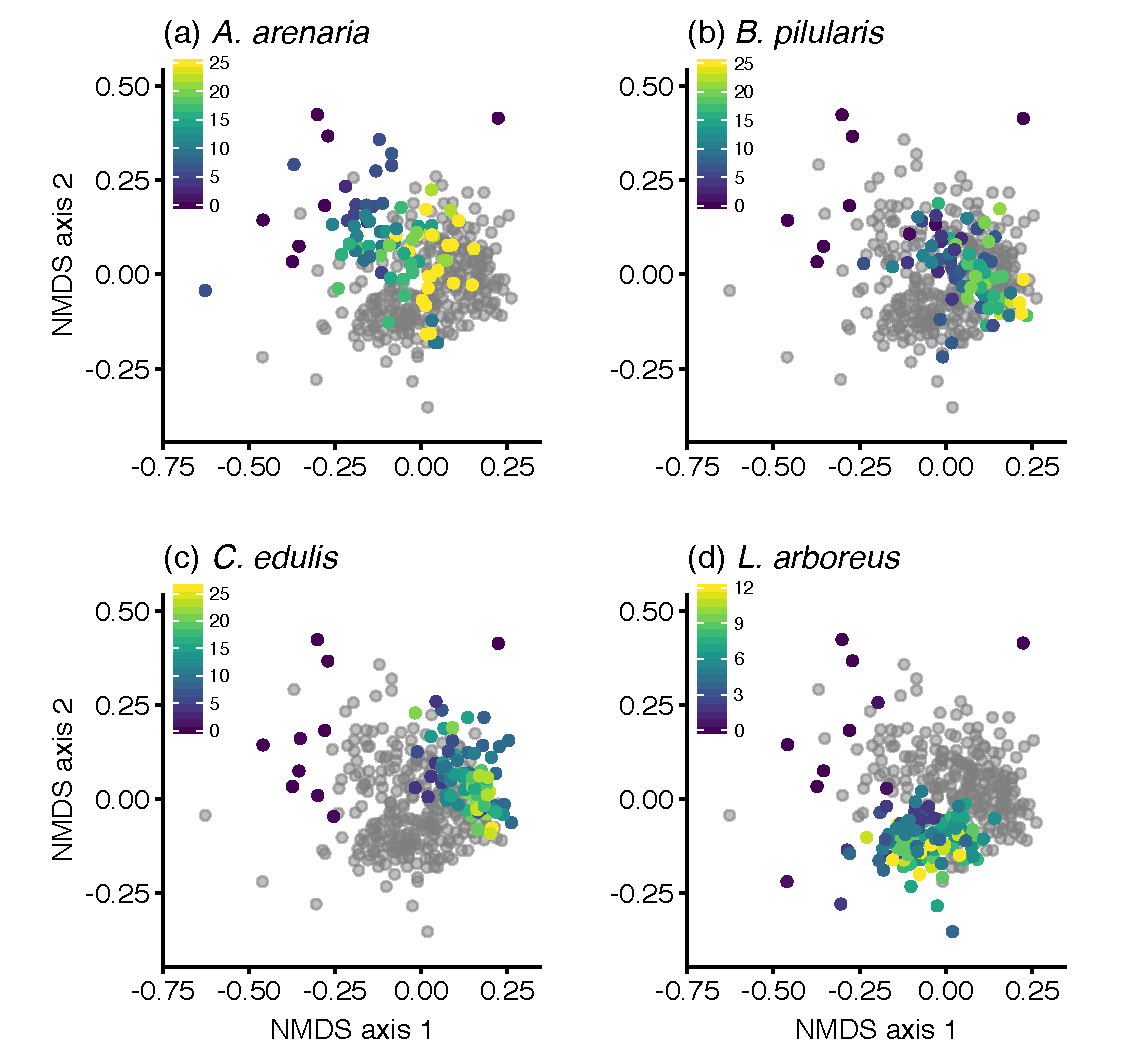
\includegraphics[width=14cm]{Chapter6/Composition_Fungi_Age.pdf}}
	\caption[Fungal community composition as a function of plant species and the age of plant individuals.]
		{\hspace{1mm} 
		Fungal community composition as a function of plant species and the age of plant individuals. Each panel highlights one focal plant species on the NMDS ordination plot of all fungal communities. Fungal communities associated with the focal species are color-coded by individual plant age, whereas the other three species are in gray. Purple to yellow represent the age gradient from young to old, with species-specific minimum and maximum age. (a) \textit{A. arenaria}; (b) \textit{B. pilularis}; (c) \textit{C. edulis}; (d) \textit{L. arboreus}. 
		Statistics were performed at the plant individual level, but for visualization purpose each point represents the fungal community of one soil sample. Note that dark purple points that appeared in all panels represent fungal communities associated with bare sand. See the same ordination plot but color-coded with species identity in Fig.~\ref{fig:BothComposition}a.}
	\label{fig:FunComposition}
\end{figure}



\newpage
\begin{figure}[h]
	\centering
	\makebox[\textwidth][c]{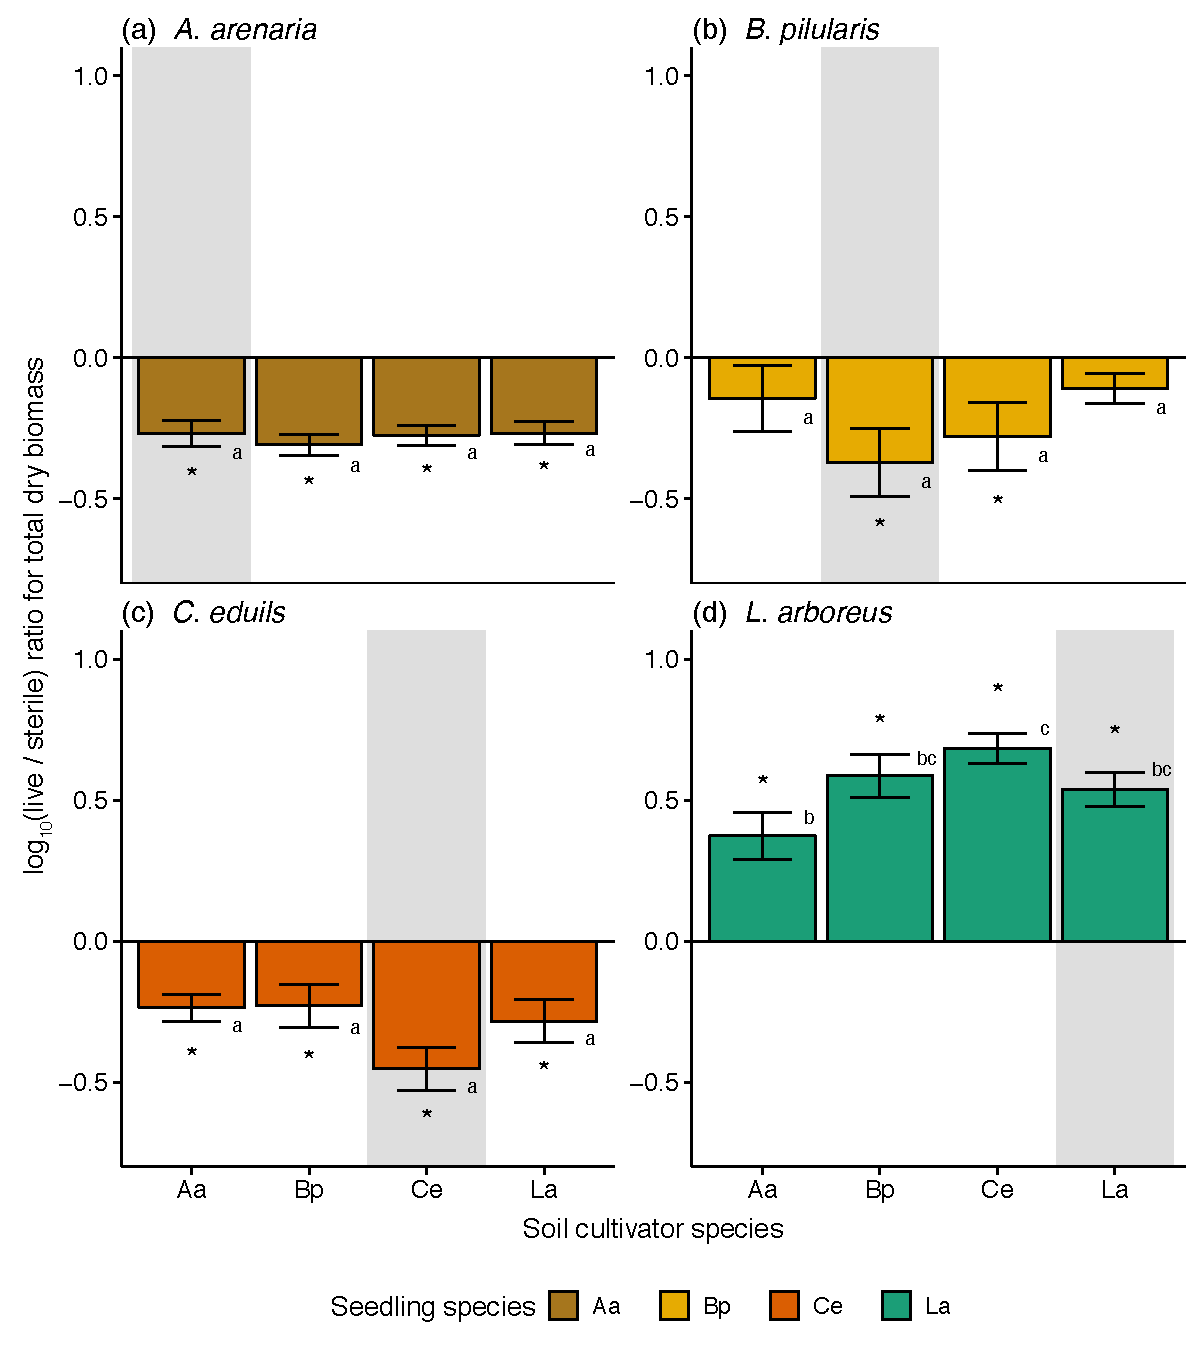
\includegraphics[width=14cm]{Chapter6/LiveSterRatioBarplot_Revised.pdf}}
	\caption[Mean ($\pm$ SE) microbial effects for each plant species in soils conditioned by different plants, neglecting the effects of soil conditioning length.]
		{\hspace{1mm} 
		Mean ($\pm$ SE) microbial effects for each plant species in soils conditioned by different plants, neglecting the effects of soil conditioning length. 
		(a) \textit{A. arenaria} (brown); (b) \textit{B. pilularis} (yellow); (c) \textit{C. edulis} (orange); (d) \textit{L. arboreus} (green). 
		The x-axis represents the plant species that conditioned the soil: \textit{A. arenaria} (Aa), \textit{B. pilularis} (Bp), \textit{C. edulis} (Ce), and \textit{L. arboreus} (La). The y-axis represents the microbial effects, defined as the log-ratio of plant total biomass in live soil and sterile soil, imposed by the soil host species. 
		Shaded bars represent conspecific microbial effects. Asterisks indicate microbial effects that are significantly different from zero, and different letters represent significant difference among the plant $\times$ soil host species combinations.}
	\label{fig:PSFBar}
\end{figure}



\newpage
\begin{figure}[h]
	%\vspace*{-1.0cm}
	\centering
	\makebox[\textwidth][c]{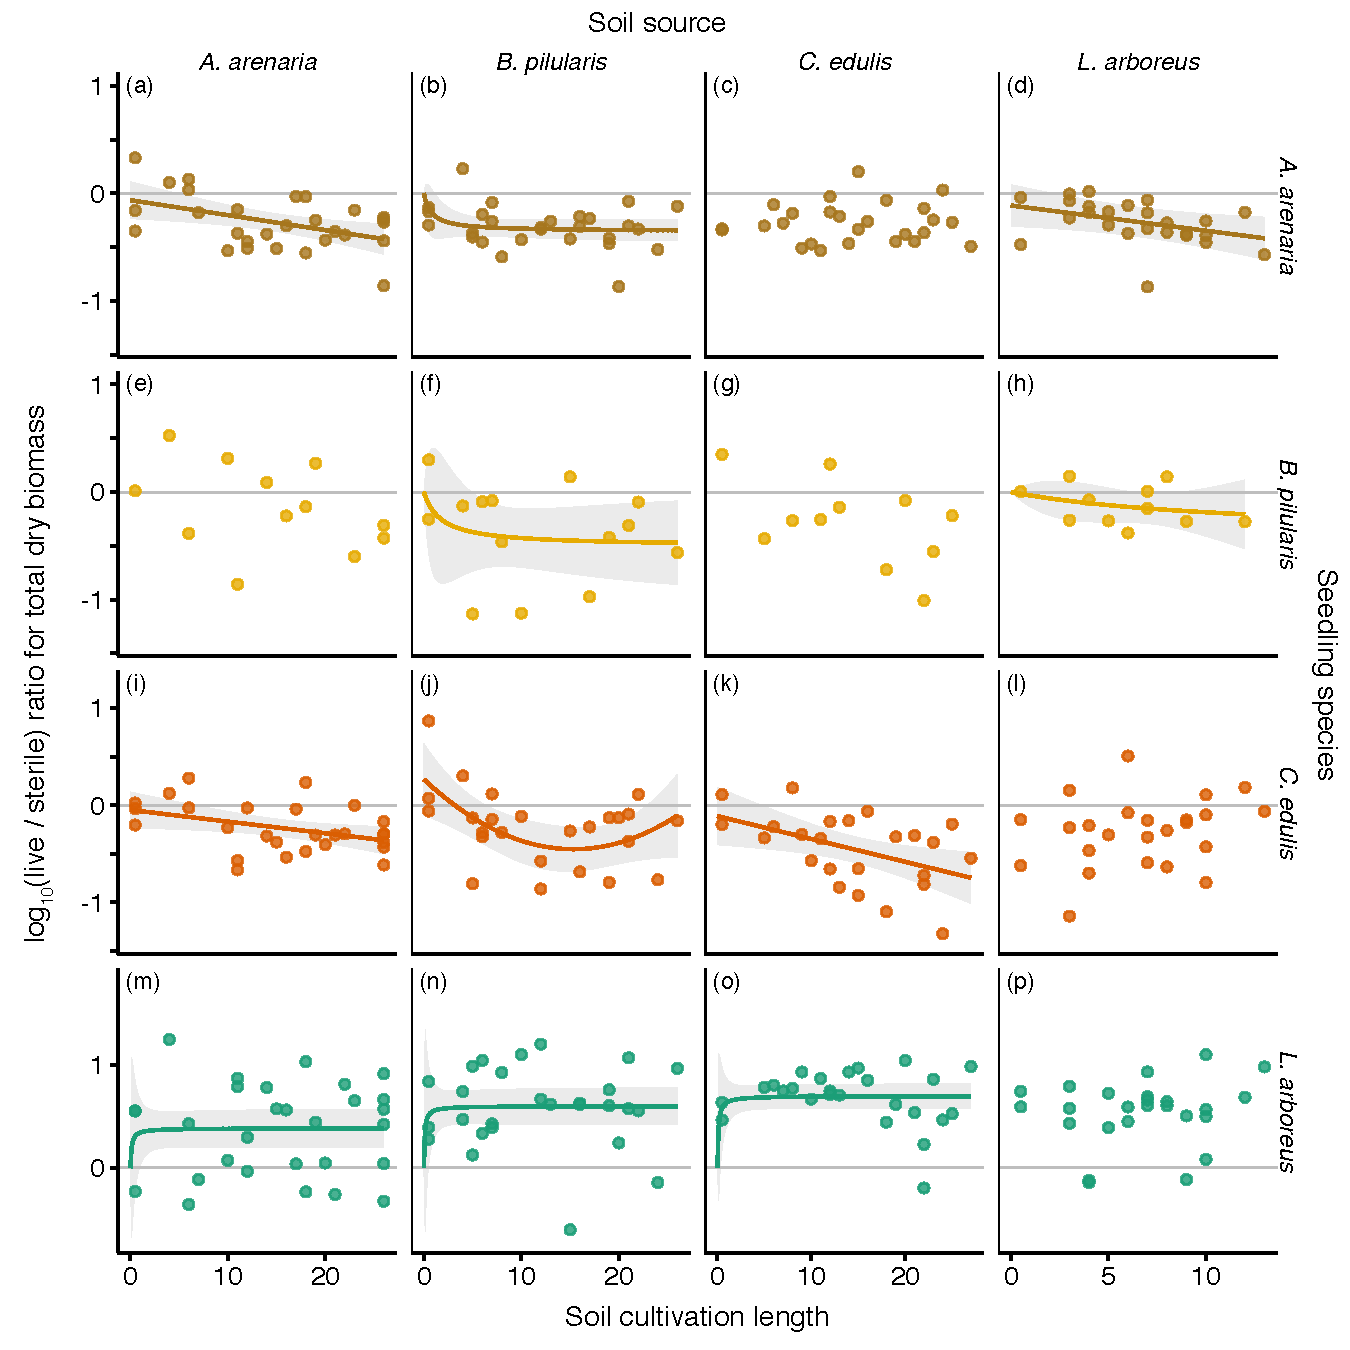
\includegraphics[width=14cm]{Chapter6/TemporalLiveSterRatio_Saturating_Revised.pdf}}
	\caption[Temporal trends of microbial effects for each plant $\times$ soil host species combination.]
		{\hspace{1mm} 
		Temporal trends of microbial effects for each plant (row) $\times$ soil host species (column) combination.
		Each point represents the microbial effect generated by soils collected from one plant individual.
		The x-axis represents the age of the plant individual that conditioned the soil, with maximum age up to 25 years old for \textit{A. arenaria} (first column), \textit{B. pilularis} (second column), and \textit{C. edulis} (third column), and up to 13 years old for \textit{L. arboreus} (fourth column). The y-axis represents the microbial effects imposed by the conditioning species, defined as the log-ratio of plant total biomass in live soil and sterile soil. The horizontal gray line in each panel represents no microbial effects.
		Colors/rows represent different plant species: \textit{A. arenaria} (brown, first row), \textit{B. pilularis} (yellow, second row), \textit{C. edulis} (orange, third row), and \textit{L. arboreus} (green, fourth row). The first three rows are plotted on the same scale.
		For each plant $\times$ soil host species combination, a fitted temporal trend line (and 95$\%$ confidence interval) is added if the length of soil conditioning affected the microbial effects (see main text for model fitting procedure).
		Note for combinations where the length of soil conditioning had little influence (i.e., no fitted trend line was added), its time-averaged microbial effects might still be significantly different from zero (see Fig.~\ref{fig:PSFBar}).}
	\label{fig:PSFTemporal}
\end{figure}



\newpage
\begin{figure}[h]
	\centering
	\makebox[\textwidth][c]{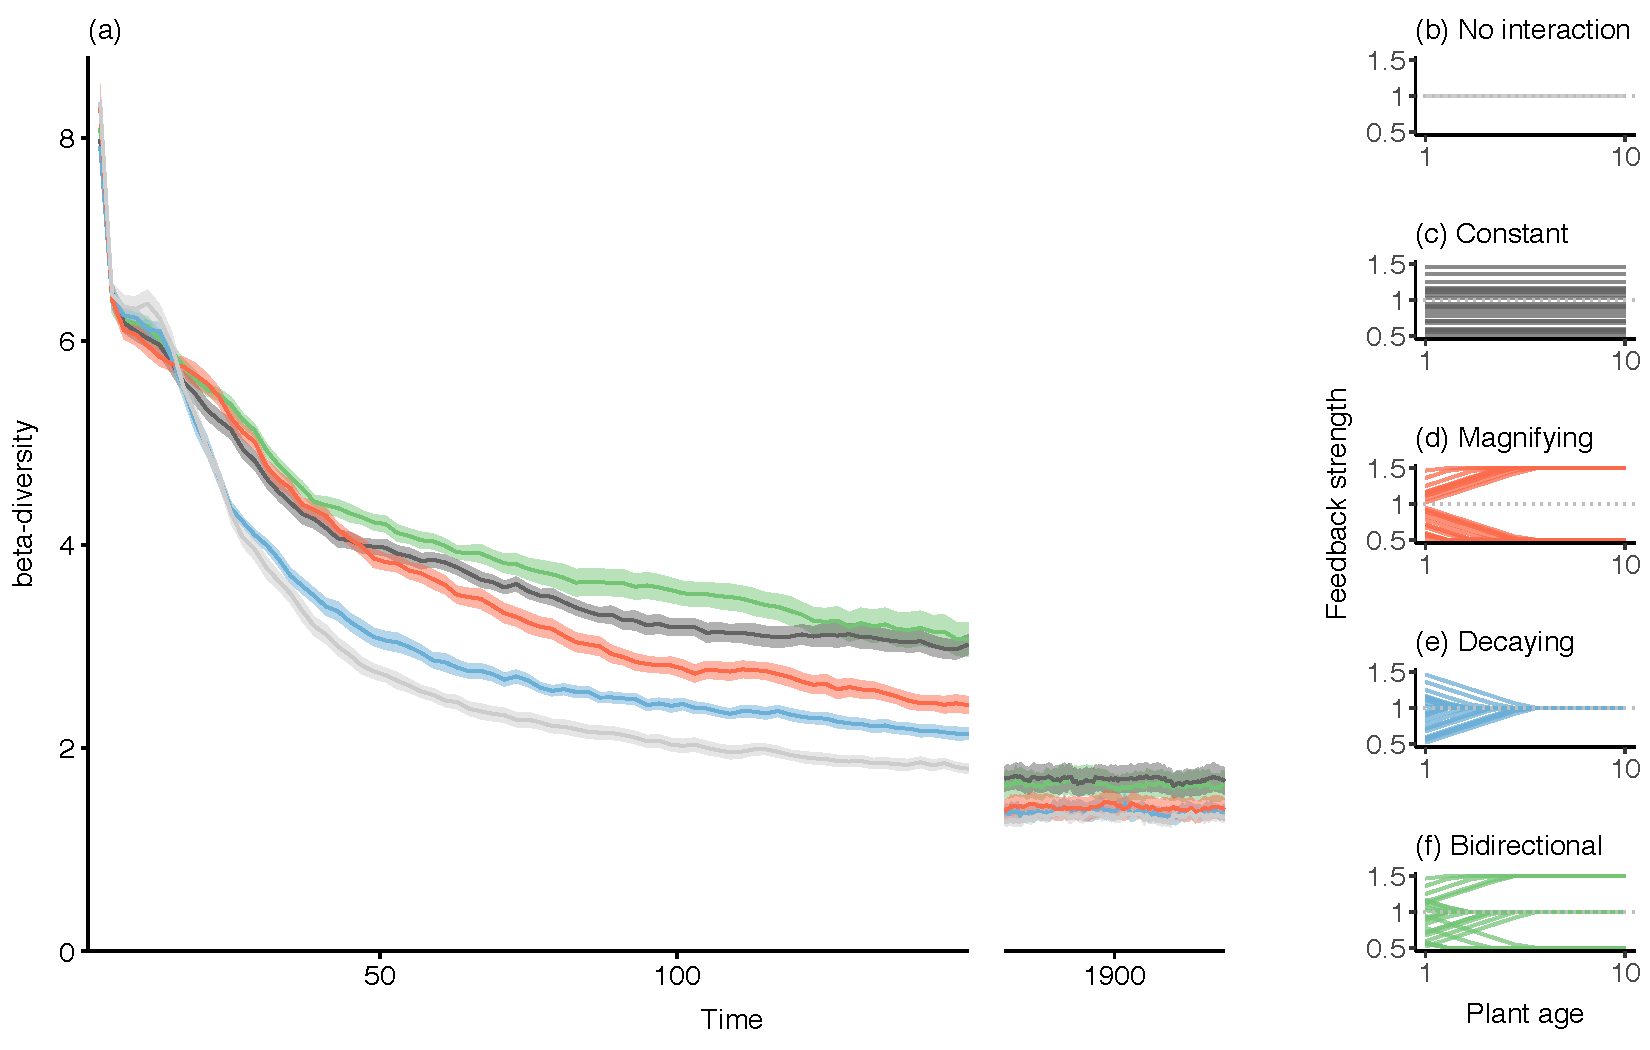
\includegraphics[width=15cm]{Chapter6/Simulation_ComplexPSF_Aggregate.pdf}}
	\caption[Simulated community convergence patterns under different temporal development scenarios of the underlying plant--soil microbe interactions.]
		{\hspace{1mm} 
		Simulated community convergence patterns under different temporal development scenarios of the underlying plant--soil microbe interactions.
		(a) Temporal trends of beta-diversity (mean $\pm$ SE, $n = 20$) among the 10 simulated patches for five different plant--soil microbe interaction scenarios. (b)--(f) Schematic diagrams of the five different scenarios in (a), demonstrating how the interaction strength changes with the age of the conditioning individual.
		(b) No plant--soil microbe interactions (light gray); (c) Plant--soil microbe interactions that are independent to plant age (black); (d) Magnifying interaction strengths that intensify to their biological extremes with increasing plant age (orange); (e) Decaying interaction strengths that attenuate to one with increasing plant age (blue); (f) Bidirectionally varying interaction strengths that either intensify or attenuate with increasing plant age (green). See Appendix E.1 for detailed model description.}
	\label{fig:SimulationComplexPSF}
\end{figure}


